\documentclass[letterpaper, 12pt]{article}

\usepackage{geometry}
 \geometry{
 letterpaper,
 total={170mm,257mm},
 left=20mm,
 top=20mm,
 bottom=20mm
 }
\usepackage{graphicx} % Required for inserting images
\usepackage{authblk}
\usepackage{amssymb}
\usepackage{lipsum}
\usepackage{float}
\usepackage{times}
\usepackage{amsmath}
\usepackage[format=plain,
            labelfont={bf,it},
            textfont=it]{caption}
\captionsetup{justification=raggedright,singlelinecheck=false}
\usepackage{ragged2e}
\usepackage{longtable}
\usepackage{comment}
\usepackage{setspace}
\usepackage{fancyhdr}
\usepackage{titlesec}
\usepackage[hyperindex,breaklinks]{hyperref}
\hypersetup{
    colorlinks=true,
    linkcolor=blue,
    filecolor=magenta,      
    urlcolor=blue,
    pdftitle={Overleaf Example},
    pdfpagemode=FullScreen,
    }
% \usepackage{background} % add COSIG logo to page
\usepackage[T1]{fontenc}
\usepackage{helvet}
\renewcommand{\familydefault}{\sfdefault}
\pagenumbering{gobble}
\usepackage[skip=10pt plus1pt, indent=40pt]{parskip}

\titlespacing*{\section}
{0pt}{1.5ex plus 1ex minus .2ex}{1.3ex plus .2ex}

\renewcommand\Authfont{\fontsize{12}{14.4}\selectfont}
\renewcommand\Affilfont{\fontsize{9}{10.8}\itshape}
 
\begin{document}
\flushleft

\includegraphics[width=0.5\textwidth]{img/home/241017_final_logo_mockup.png}

\addcontentsline{toc}{part}{Mathematics and statistics}
\section*{Evaluating the performance of binary classifiers}
\addcontentsline{toc}{section}{Evaluating the performance of binary classifiers}
\textit{Last updated: 7 May 2025}

A \href{https://en.wikipedia.org/wiki/Classification_rule}{classifier} is an procedure that sorts objects in a population into classes. A binary classifier sorts a population into two classes. Some examples of binary classifiers include:

\begin{itemize}
    \setlength\itemsep{-0.5em}
    \item a computer vision program that predicts if an image depicts a horse or does not depict a horse
    \item a medical diagnostic criteria (has a diseases versus does not have a disease)
    \item an algorithm that predicts whether or not it will rain on a given day
    \item a statistical test (null hypothesis rejected versus null hypothesis not rejected)
\end{itemize}

Usually, one class is labeled the positive condition and the other class is labeled the negative condition. Each object in the population is either an actual negative (N) or an actual positive (P) and each prediction for that object is either a predicted positive (PP) or predicted negative (PN). Then after the class is predicted by the classifier, each object is one of the following:

\begin{itemize}
    \setlength\itemsep{-0.5em}
    \item \textbf{A true positive (TP):} P and PP
    \item \textbf{A true negative (TN):} N and PN
    \item \textbf{A false positive (FP, a \href{https://en.wikipedia.org/wiki/Type_I_and_type_II_errors}{Type I error}):} N and PP
    \item \textbf{A false negative (FN, a \href{https://en.wikipedia.org/wiki/Type_I_and_type_II_errors}{Type II error}):} P and PN
\end{itemize}

The number of objects in the population in each outcome is typically represented in a \href{https://en.wikipedia.org/wiki/Confusion_matrix}{confusion matrix}.

\begin{figure}[h!tbp]
    \centering
    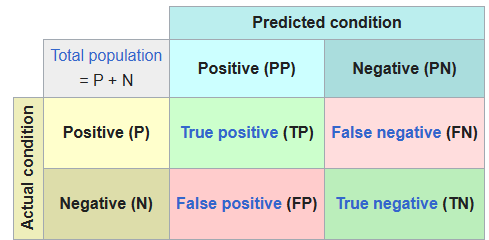
\includegraphics[width=0.75\textwidth]{img/classifier_eval/confusion_matrix.png}
    \caption*{A confusion matrix. Adapted from \href{https://en.wikipedia.org/wiki/Confusion_matrix}{Wikipedia}.}
\end{figure}

For example, the following classes and predicted classes (True, T and False, F):

\begin{center}
\begin{tabular}{|p{2.0cm}|p{2.0cm}|p{2.0cm}|}
\hline
     \textbf{Actual Class} & \textbf{Predicted Class} & \textbf{Outcome}\\ \hline\hline
     T & T & TP \\\hline
     T & T & TP \\\hline
     T & T & TP \\\hline
     F & F & TN \\\hline
     F & F & TN \\\hline
     F & F & TN \\\hline
     F & F & TN \\\hline
     F & T & FP \\\hline
     F & T & FP \\\hline
     T & F & FN \\\hline
\end{tabular}
\end{center}

would yield the following confusion matrix:

\begin{center}
\begin{tabular}{p{1.0cm}|p{1.0cm}|p{1.0cm}}
    & \textbf{PP} & \textbf{PN}
     \\ \hline
     \textbf{P} & 3 & 1 \\\hline
     \textbf{N} & 2 & 4 \\
\end{tabular}
\end{center}

A number of metrics can be calculated to quantify how well a classifier performs. Many are summarized in the figure below. This guide summarizes some of the most popular metrics. These metrics can be calculated with for any 2x2 confusion matrix. 

Sometimes scientific articles will report a value for a metric that does not match the corresponding confusion matrix or will report impossible values for a metric (such as accuracy score above 1.0).

\begin{figure}[h!tbp]
    \centering
    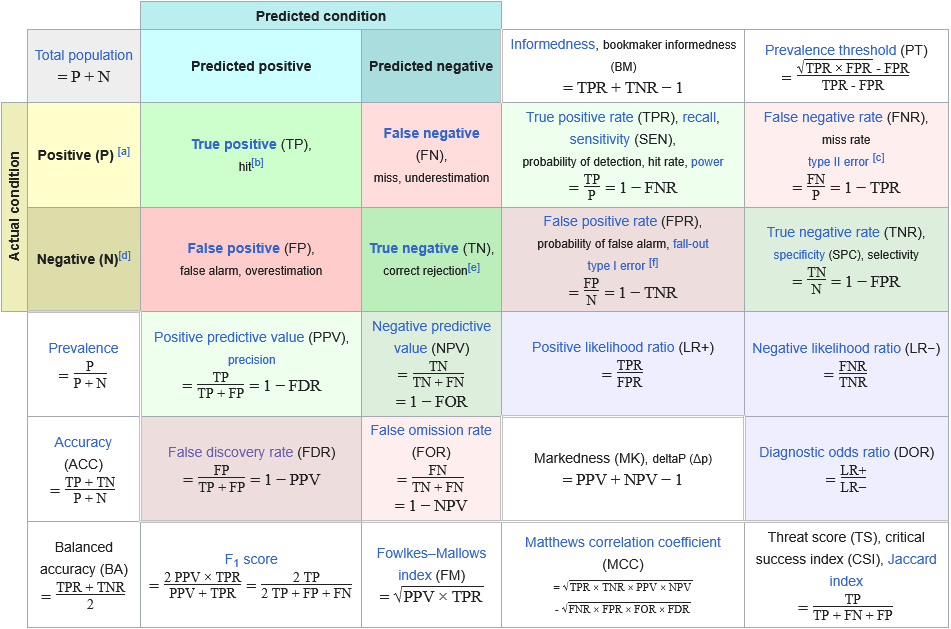
\includegraphics[width=\textwidth]{img/classifier_eval/extended_confusion_matrix.png}
    \caption*{An extended confusion matrix detailing various metrics for evaluating binary classifiers. Adapted from \href{https://en.wikipedia.org/wiki/Evaluation_of_binary_classifiers}{Wikipedia}.}
\end{figure}

\pagebreak

\subsection*{True positive rate (TPR)/recall/sensitivity}

True positive rate (TPR), commonly called recall or sensitivity, is the likelihood that an an actual positive is predicted as a positive. In the context of hypothesis testing, this metric is often described as power. For a binary classifier, TPR will always be greater than or equal to 0.0 and less than or equal to 1.0.

$$\textrm{TPR} = \frac{\textrm{TP}}{\textrm{P}}$$

\subsection*{False negative rate (FNR)}

False negative rate (FNR), also called miss rate, is the likelihood that an actual positive is predicted as a negative. TPR and FNR invariably sum to 1.0. For a binary classifier, FNR will always be greater than or equal to 0.0 and less than or equal to 1.0.

$$\textrm{FNR} = \frac{\textrm{FN}}{\textrm{P}} = 1 - \textrm{TPR}$$

\subsection*{False positive rate (FPR)}

False positive rate (FPR) is the likelihood that an actual negative is predicted as a positive. For a binary classifier, FPR score will always be greater than or equal to 0.0 and less than or equal to 1.0.

$$\textrm{FPR} = \frac{\textrm{FP}}{\textrm{N}}$$

\subsection*{True negative rate (TNR)/specificity}

True negative rate (TNR), commonly called specificity, is the likelihood that an actual negative is predicted as a negative. TNR and FPR invariably sum to 1.0. For a binary classifier, TNR will always be greater than or equal to 0.0 and less than or equal to 1.0.

$$\textrm{FNR} = \frac{\textrm{FP}}{\textrm{N}} = 1 - \textrm{FPR}$$

\subsection*{Positive predictive value (PPV)/precision}

Positive predictive value (PPV), commonly called precision, describes the likelihood that any predicted positive is a true positive. For a binary classifier, PPV will always be greater than or equal to 0.0 and less than or equal to 1.0.

$$\textrm{PPV} = \frac{\textrm{TP}}{\textrm{PP}} = \frac{\textrm{TP}}{\textrm{TP} + \textrm{FP}}$$

\subsection*{False discovery rate (FDR)}

False discovery rate (FDR) describes the likelihood that any predicted positive is a false positive. PPV and FDR invariably sum to 1.0. For a binary classifier, FDR will always be greater than or equal to 0.0 and less than or equal to 1.0.

$$\textrm{FDR} = \frac{\textrm{FP}}{\textrm{PP}} = \frac{\textrm{FP}}{\textrm{TP} + \textrm{FP}} = 1 - \textrm{PPV}$$

\subsection*{Negative predictive value (NPV)}

Negative predictive value (NPV) describes the likelihood that any predicted negative is a true negative. For a binary classifier, NPV will always be greater than or equal to 0.0 and less than or equal to 1.0.

$$\textrm{NPV} = \frac{\textrm{TN}}{\textrm{PN}} = \frac{\textrm{TN}}{\textrm{TN} + \textrm{FN}}$$

\subsection*{False omission rate (FOR)}

False omission rate (FOR) describes the likelihood that any predicted negative is a false negative. NPV and FOR invariably sum to 1.0. For a binary classifier, FOR will always be greater than or equal to 0.0 and less than or equal to 1.0.

$$\textrm{FOR} = \frac{\textrm{FN}}{\textrm{PN}} = \frac{\textrm{FN}}{\textrm{TN} + \textrm{FN}}$$

\subsection*{Accuracy}

Accuracy measures the overall predictive performance of a binary classifier. It is the likelihood that a predicted class is correct. For a binary classifier, accuracy will always be greater than or equal to 0.0 and less than or equal to 1.0.

$$\textrm{Accuracy} = \frac{\textrm{TP} + \textrm{TN}}{\textrm{P} + \textrm{N}}$$

\subsection*{Balanced accuracy}

Balanced accuracy also measures the overall predictive performance of a binary classifier and is generally used when there is a large imbalance in classes (i.e., there are many more actual negatives than actual positives or vice versa). It is the \href{https://en.wikipedia.org/wiki/Arithmetic_mean}{arithmetic mean} of TPR (sensitivity) and TNR (specificity). Thus, balanced accuracy must fall between the values of TPR and TNR. For a binary classifier, balanced accuracy will always be greater than or equal to 0.0 and less than or equal to 1.0.

$$\textrm{Balanced Accuracy} = \frac{\textrm{TPR} + \textrm{TNR}}{2}$$

\subsection*{F1 score}

F1 score, also called F-score or F-measure, is a composite score for evaluating the overall performance of a binary classifier. It is the \href{https://en.wikipedia.org/wiki/Harmonic_mean}{harmonic mean} of PPV (precision) and TPR (recall). Thus, F1 score must fall between the values of PPV and TPR. For a binary classifier, F1 score will always be greater than or equal to 0.0 and less than or equal to 1.0.

$$\textrm{F1} = \frac{1}{\frac{1}{PPV} + \frac{1}{\textrm{TPR}}} = \frac{2 \cdot \textrm{TPR} \cdot \textrm{PPV}}{\textrm{TPR} + \textrm{PPV}} = \frac{2 \cdot \textrm{TP}}{2 \cdot \textrm{TP} + \textrm{FP} + \textrm{FN}}$$

\subsection*{Matthews Correlation Coefficient (MCC)}

The \href{https://en.wikipedia.org/wiki/Phi_coefficient}{Matthews Correlation Coefficient} is a composite score for evaluating the overall performance of a binary classifier. For a binary classifier, MCC will always be greater than or equal to -1.0 and less than or equal to 1.0.

\begin{align*} 
\textrm{MCC} &= \sqrt{\textrm{TPR} \cdot \textrm{TNR} \cdot \textrm{PPV} \cdot \textrm{NPV}} - \sqrt{\textrm{FNR} \cdot \textrm{FPR} \cdot \textrm{FOR} \cdot \textrm{FDR}}\\ 
 &= \frac{\textrm{TP}\cdot\textrm{TN}-\textrm{FP}\cdot\textrm{FN}}{\sqrt{ (\textrm{TP}+\textrm{FP})\cdot(\textrm{TP}+\textrm{FN})\cdot(\textrm{TN}+\textrm{FP})\cdot(\textrm{TN}+\textrm{FN}) }}\
\end{align*}

\pagebreak

\subsection*{Example 1: Unclear use of binary classifier, inconsistent evaluation metrics}

\href{https://doi.org/10.1007/s12665-024-11768-y}{Mao et al. (2024)} report on an algorithm that predicts the elasticity modulus of sedimentary rocks. Throughout the text the authors imply that they evaluated the performance of the algorithm with confusion matrices and binary classifier metrics. However, it is unclear what binary variable was being predicted (elasticity modulus is a continuous variable). Furthermore, in Table 3, there are several instances where reported values for F1 score are inconsistent with the reported values of precision and recall. In one instance, precision is reported as 0.65 and recall is reported as 0.70, which implies an F1 score of $\sim$0.67 (the harmonic mean of precision and recall). However, the F1 score is reported as 0.70. In another instance, precision and recall are both reported as 0.97, but F1 score is reported as 0.95 (F1 score must fall between precision and recall).

\begin{figure}[h!tbp]
    \centering
    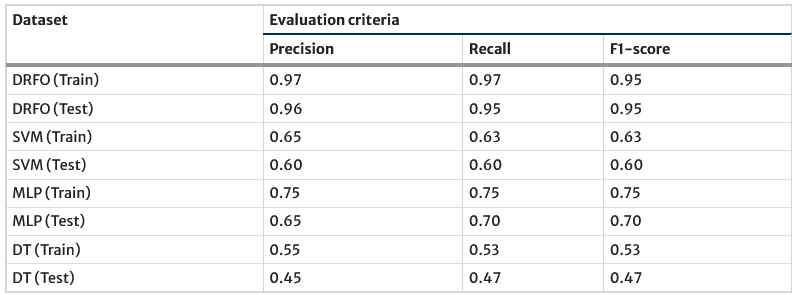
\includegraphics[width=\textwidth]{img/classifier_eval/mao_et_al_table_3.png}
    \caption*{Adapted from Table 3 of \href{https://doi.org/10.1007/s12665-024-11768-y}{Mao et al. (2024)}.}
\end{figure}

\pagebreak

\subsection*{Example 2: Incorrect F1 scores}

\href{https://doi.org/10.1038/s41598-023-41314-y}{Lihore et al. (2023)} report on a model that predicts Parkinson's disease. In Table 5, several F1 scores are inconsistent with their corresponding precision and recall values. For instance, where precision is reported as 0.754 and recall is reported as 0.764, the F1 score is reported as 0.778 when it should be $\sim$0.759. The article was \href{https://doi.org/10.1038/s41598-024-78418-y}{retracted} in 2024. The retraction notice states ``analysis of the data presented in the Article found that the F-score shown in Table 5 appears to be incorrectly calculated''.

\begin{figure}[h!tbp]
    \centering
    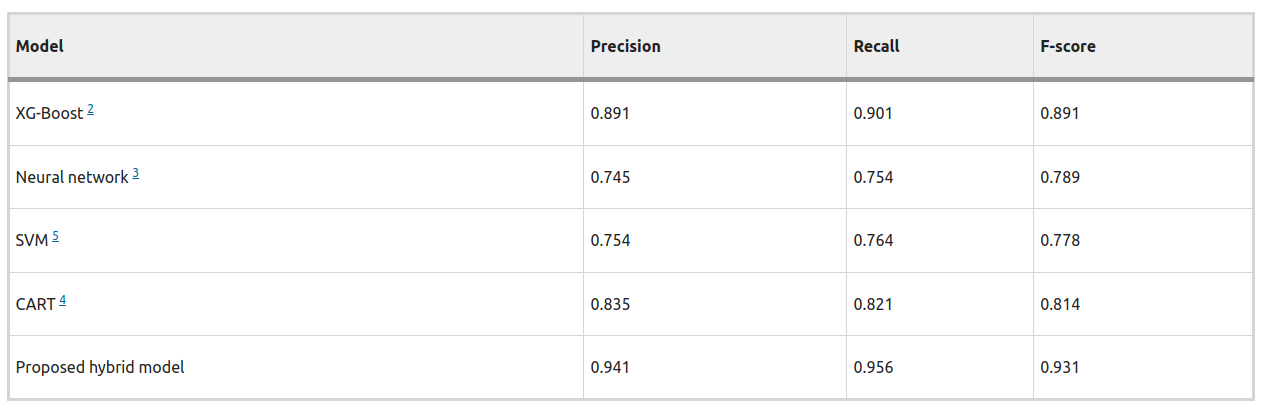
\includegraphics[width=\textwidth]{img/classifier_eval/lihore_f1.png}
    \caption*{Adapted from Table 5 of \href{https://doi.org/10.1038/s41598-023-41314-y}{Lihore et al. (2023)}.}
\end{figure}

\subsection*{Example 3: Impossible accuracy, F1, precision and recall scores}

\href{https://doi.org/10.1109/IC3I59117.2023.10397896}{Sharma et al. (2023)} report on models for predicting disease. At many points throughout the text, the authors report values for evaluation metrics that are not possible, such as when they claim that a model ``excels with an f1
score of 0.11 and an accuracy of 1.76'' (accuracy cannot be greater than 1.0). Table 2 reports several values for precision, recall and F1 score greater than 1.0, also impossible for a binary classifier. An \href{https://doi.org/10.1109/IC3I59117.2023.10703725}{expression of concern} was issued for this article in 2024.

\begin{figure}[h!tbp]
    \centering
    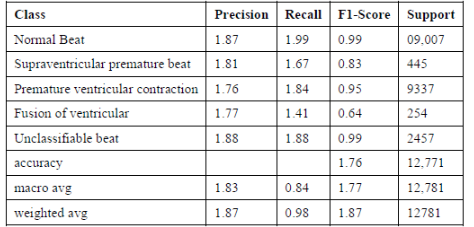
\includegraphics[width=0.8\textwidth]{img/classifier_eval/sharma_et_al_table_2.png}
    \caption*{Adapted from Table 2 of \href{https://doi.org/10.1109/IC3I59117.2023.10397896}{Sharma et al. (2023)} .}
\end{figure}

\subsection*{Additional resources}

\begin{itemize}
    \setlength\itemsep{-0.5em}
    \item \href{https://doi.org/10.1016/j.aci.2018.08.003}{``Classification assessment methods'' (2020)}
    \item \href{https://doi.org/10.1186/s12864-019-6413-7}{``The advantages of the Matthews correlation coefficient (MCC) over F1 score and accuracy in binary classification evaluation'' (2020)}
\end{itemize}


\end{document}